\documentclass[twoside]{article}

\usepackage[math]{kurier}
\usepackage[sc]{mathpazo}
\renewcommand{\sfdefault}{kurier}

\usepackage[boxruled]{algorithm2e}
\usepackage[utf8]{inputenc}
\usepackage[backend=biber]{biblatex}
\usepackage[english]{babel}
\usepackage[english]{babel}
\usepackage[autostyle]{csquotes}
\usepackage{placeins}
\usepackage[backend=biber]{biblatex}
\bibliography{./lecture_15_biblio.bib}

\usepackage{tikz,pgfplots}
\usepackage{xcolor, colortbl}
\usepackage{array}
\usepackage[boxruled]{algorithm2e}


\usepackage{graphics}
\usepackage{graphicx}
\usepackage{subcaption}
\usepackage{amsmath}
\usepackage{float}
\setlength{\oddsidemargin}{0.25 in}
\setlength{\evensidemargin}{-0.25 in}
\setlength{\topmargin}{-0.6 in}
\setlength{\textwidth}{6.5 in}
\setlength{\textheight}{8.5 in}
\setlength{\headsep}{0.75 in}
\setlength{\parindent}{0 in}
\setlength{\parskip}{0.1 in}
\DeclareMathOperator*{\argmin}{arg\,min}


\newcounter{lecnum}
\renewcommand{\thepage}{\thelecnum-\arabic{page}}
\renewcommand{\thesection}{\thelecnum.\arabic{section}}
\renewcommand{\theequation}{\thelecnum.\arabic{equation}}
\renewcommand{\thefigure}{\thelecnum.\arabic{figure}}
\renewcommand{\thetable}{\thelecnum.\arabic{table}}


\newcommand{\lecture}[3]{
   \pagestyle{myheadings}
   \thispagestyle{plain}
   \newpage
   \setcounter{lecnum}{#1}
   \setcounter{page}{1}
   \noindent
   \begin{center}
   \framebox{
      \vbox{\vspace{2mm}
    \hbox to 6.28in { {\bf \sffamily AA 274: Principles of Robotic Autonomy
                        \hfill Winter 2019} }
       \vspace{4mm}
       \hbox to 6.28in { {\sffamily{\Large \hfill Lecture #1: #2  \hfill}} }
       \vspace{2mm}
       % \hbox to 6.28in { {\it \hfill Scribes: #4} }
      \vspace{2mm}}
   }
   \end{center}
   \markboth{Lecture #1: #2}{Lecture #1: #2}

   \vspace*{4mm}
}


%%%%%%%%%%%%%%%%%%%%%%%%%%
%document
\begin{document}
\nocite{pavone}
\nocite{siegwart}
\nocite{bertsekas}
\nocite{lavalle}

\lecture{15}{Combinatorial Motion Planning}{}

\section{Introduction}

A robot must show competence in reaching its goal position as efficiently as possible based on its knowledge and sensor values given a series of goal positions and a map of its environment. This task gives rise to the navigation or motion planning problem.

\textbf{Robot motion planning}: compute a sequence of actions that drives a robot from an initial condition to a terminal condition while avoiding obstacles, satisfying kinematic and dynamic constraints, and possibly optimizing an objective function.

Some examples of common motion planning problems may include steering autonomous vehicles, controlling humanoid robots, protein docking, and surgery planning.

\subsection{ History }

The problem of motion planning was formally defined in the 1970s as mobile robots became more prevalent in industries. However, exact combinatorial solutions in discrete configuration spaces were not developed until the 1980s with the introduction of Breadth-First Search and Depth-First Search algorithms. Grid-based search algorithms such as A* and D* which was developed by Anthony Stentz followed in the mid-1990s \cite{bertsekas}. These methods worked well for simple motion planning problems but were subject to the curse of dimensionality for planning in high-dimensional state spaces. To address this challenge,
sampling-based methods, notably Probability Road-Maps (PRM) and Rapidly-Exploring Random Trees (RRT), were developed in the late 1990s and deployed on real-time systems in the 2000s \cite{lavalle}. With the increasing complexity of robotic systems, solving motion planning problems in real-time has become a significant challenge. Hence, current research has focused on speeding up sampling-based methods through lazy dynamic programming and massive parallelization of search algorithms. 

\section{Configuration-Space}
In the context of robotic motion planning, we will first create a simple problem setup to define the variables of interest and introduce the proper nomenclature. First, consider a workspace defined in 2D, $ W \subseteq R^2$, which effectively describes the world that is occupied by the robot, the obstacles, and potentially other agents in the system. Within this workspace, we define the robot as a rigid polygon, and we introduce the set of obstacles $O \subset W$ as a subset of the workspace shown in Fig 15.1.

The rigid robot can be translated or rotated according to its own kinematic constraints. With these definitions established, we can qualitatively define the robotic motion planning problem as:

\begin{figure}[h]
\begin{center}
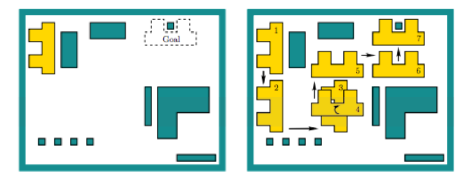
\includegraphics{fig15_1.PNG}
\caption{2D Workspace}
\end{center}
\end{figure}

\textbf{Problem Statement}: Compute the sequence of movements to go from a given initial placement of the robot to a desired goal placement such that the robot never touches the obstacle regions.

While the robot motion planning problem is described in a physically intuitive ”real-world” setting (e.g., the 2D planar workspace described above), it is vital to map the problem into another space, denoted as the configuration (C-) space. The configuration space is simply the space containing the degrees of freedom of the robot. Returning to our simple example highlighted above, the configuration space contains
the translational degrees of freedom and the rotational degrees of freedom of the robot. In this way, the 2D path planning problem in physical space is cast as a 3D path planning problem in the configuration space, with two dimensions describe the translational modes of the trajectory and one degree of freedom capturing the rotational mode of the trajectory in the planar workspace.
 
Formally, the degrees of freedom for our rigid polygon robot, R R2, is the set of generalized coordinates, $q = (xt, yt, q)$, where (xt, yt) R2 are the translational coordinates, and q is the rotational coordinate. Accordingly, the configuration space consists of every combination of q which yields a unique robot placement (in this case a subset of R3). An important distinction must be made for the generalized coordinate describing the rotational degree of freedom; namely, q and q2pk, k2 Z describe equivalent attitudes. The configuration space in this case is actually in R2 S1, where S1 is the manifold which contains the angular displacement variable and includes the aforementioned ”equivalence” between angles that differ by integer multiples of 2p. If we relax the planar restriction in our working example, the angular orientation coordinates of the robot would instead be in the manifold S3. The importance of this distinction is highlighted with a simple example: consider a robot that has a current heading of q = 3p/2 rads, and we want to reconfigure the robot to heading qg = 0 subject to the constraint of avoiding a C-space obstacle at q = p. The geometry of this problem is highlighted in Figure 15.2. Now, if the equivalence between the angles 0 and 2p is not established in the definition of the configuration space, the robot would not be able to traverse a collision-free path to the desired heading in the configuration space (see red trajectory). Instead, since the configuration space is defined with respect to S1, the robot is able to achieve the desired heading (see green trajectory).

\begin{figure}[h]
\begin{center}
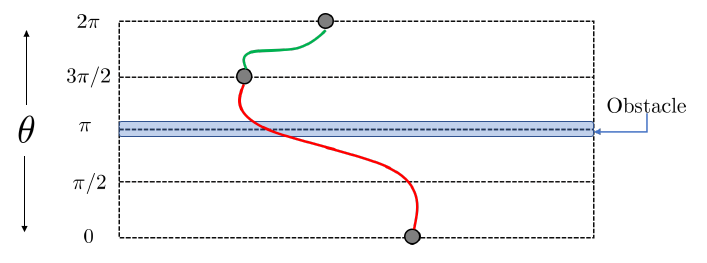
\includegraphics{fig15_2.PNG}
\caption{Example trajectory planning where the rotational degree of freedom is not described on S1 (red) and where it is described on S1 (green)}
\end{center}
\end{figure}

Note that for our simple planar workspace example, the dimensions of the physical space and the configuration space are quite similar. Instead, it is not uncommon for complicated dynamical systems (e.g., a robotic arm mounted on a spacecraft) to have configuration spaces of much higher dimension than the physical space counterpart. In these cases, mapping from physical space to configuration space is extremely
vital to the motion planning problem as it allows all constraints of the complex kinematic system to be accounted for with higher-dimensional information (i.e., more coordinates).

\subsection{ Planning in C-Space }
Now that we have introduced the necessary nomenclature and addressed the important distinction between motion planning in the real (physical) space and the configuration space, we can return to our prior problem statement and re-write it in rigorous mathematical detail. Let the set of points in the workspace that are occupied by the robot in configuration q be denoted by R(q) W. Furthermore, we can make the intuitive definition of collision-free motion as that set of all robot configurations which do not intersect the obstacle regions: $R(q)\cap O = \emptyset$. Then the formal problem statement can be re-written as: 

Problem Statement, Revisited:
Compute the continuous path: t : [0, 1] ) fq 2 CjR(q) \ O = Æg with t(0) = qI and t(1) = qG In general, we refer to the set fq 2 CjR(q) \ O = Æg as Cf ree, which represents all possible combinations of the robot’s degrees of freedom which are collision-free. A key fact here is that, while a robot occupies physical dimensions in the real space, the robotic motion is described by a simple point in the configuration space that captures the translation degrees of freedom (of the center of mass for example) and the rotational degrees of freedom of the robot. In this way, mapping to the configuration space poses the motion planning problem as a simpler problem of finding a path for a point. An illustration of this problem is highlighted in Figure 15.3. The physical dimensionality of the robot is intrinsically captured in the definition of the configuration space (in particular, in Cf ree). This property represents a key advantage
of moving to the configuration space for robotic motion planning, as it allows the same general planning problem formulation (i.e., path planning for a point) to be equally applicable to myriad dynamical systems.

\begin{figure}[H]
\begin{center}
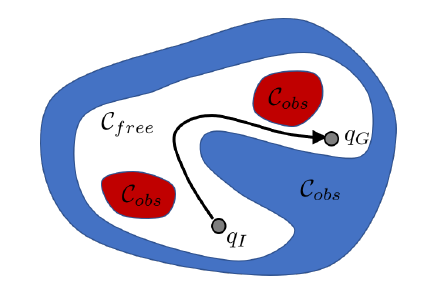
\includegraphics{fig15_3.PNG}
\caption{Robotic motion planning as a point path planning problem in C-space.}
\end{center}
\end{figure}

We now have a formal mathematical definition for the robot motion planning problem. In order to simplify the procedure, we recast the problem from the real/physical space to the configuration space. The result is that the motion planning problem now becomes a path planning problem for a single point. We have not yet, however, set up an architecture for obtaining the point path solution. In the following sections, several solution methods will be highlighted which leverage the aforementioned advantages of working in the configuration space for motion planning.

\section{Combinatorial Planning}
The goal of combinatorial planning is to find paths through the configuration space without needing approximations. For example, Figure \ref{fig:15_4} represents a point robot in a plane. The key idea is to compute a roadmap, which is a graph in which each vertex is a configuration in $C_\text{free}$ and each edge is a path through $C_\text{free}$ that connects a pair of vertices.

For low dimensional convex problems, this type of planning either provides \textit{exact} solutions or none if no feasible path exists. This can allow for better performance in some cases, compared to approximation-based methods.

\begin{figure}[H]
\begin{center}
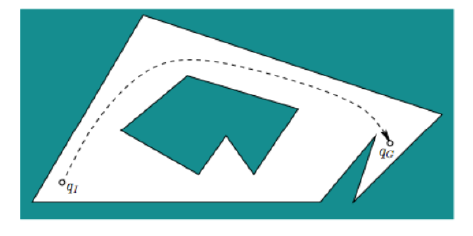
\includegraphics[width=0.6\textwidth]{fig15_4.PNG}
\caption{Combinatorial Planning}
\label{fig:15_4}
\end{center}
\end{figure}

Combinatorial Planning refers to the use of all combinations of possible states in defining the robot configuration $q$. For example, consider the configurations used above in setting up the configuration-space: $q = (x_t, y_t, \theta)$. In this case, the $x$ and $y$ position and the heading $\theta$ define a unique configuration.

Combinatorial motion planning approaches construct a roadmap, a graph $G$ which should preserve:

\begin{enumerate}
	\item \textbf{Accessiblity}: It is always possible to connect some $q$ to the roadmap. For instance, $q_I$ can be connected to $s_1$ and $q_G$ can be connected to $s_2$ on the roadmap.
	\item \textbf{Connectivity}: If there is a path between two configurations $q_I$ and $q_G$, then there exists a path on the roadmap between $s_1$ and $s_2$.
\end{enumerate}

The roadmap essentially provides a discrete representation of the continuous problem without losing any of the original connectivity information needed to solve it.

The typical approach involves cell decomposition. There are requirements that the cells be easy to traverse, the decomposition be easy to compute, and the cell adjacencies be straightforward to determine.

\section{Cell Decomposition}
In order to pick the roadmap, a discrete representation of the configuration space, the environment needs to be decomposed in a way where connectivity of the environment is captured. Cell decomposition refers to algorithms that partitions Cf ree into a finite set of regions called cells. Three properties should be satisfied by cell decomposition, to reduce motion planning problem to a graph search problem:

1. Each cell should be easy to traverse. For instance, for ideal convex cell, any points inside it must be connected by a line segment.
2. Decomposition should be easy to compute.
3. Adjacencies between cells should be straightforward to determine, in order to build the roadmap.

\subsection{2D Decomposition}
We first take a look at 2D vertical cell decomposition, which partitions Cf ree into a finite collection of 2-cells and 1-cells, where k-cell refers to a k-dimensional cell. Each 2-cell is either a trapezoid or a triangle.
Each 1-cell is a vertical segment that serves as the border of two 2-cells. Figure 15.5 shows an environment demonstrated as a configuration space, with free configuration space Cf ree represented as the white regions and obstacle space Cobs represented as the dark regions. In other words, those configurations for the robot would lead to collision. Though the planning problem is 2-dimensional, the robot configuration space is 3-dimensional, as robot heading affects whether it collides with obstacles as well.

\begin{figure}[h]
\begin{center}
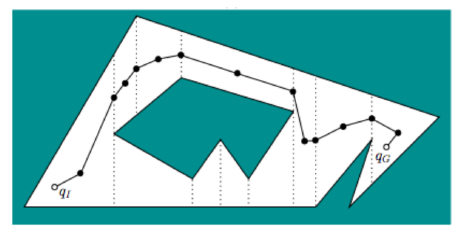
\includegraphics{fig15_5.PNG}
\caption{Example of 2D Cell Decomposition and Roadmap Extraction given qI and qG.}
\end{center}
\end{figure}

Assume the obstacle space is polygonal, then vertical cell decomposition works as follows. Let P denote the set of vertices used to define Cobs. For each vertex p 2 P, extend rays upwards and downwards through Cf ree, until Cobs is reached. Every intersection forms a cell, and thus the environment becomes a set of cells. As all cells have shapes of either triangles or trapezoids, they form convex sets. Hence, if
we put a roadmap node randomly inside a cell, all other configurations within this cell can be connected to the roadmap point. In consequence, connectivity of the environment is preserved through this cell decomposition.

Now that we have different cells that compose the environment. One possible way is to place roadmap sample point at the centroid of each cell and at midpoint of each boundary. Once the roadmap is constructed, given any initial and goal configurations qI and qG, a path can always be extracted from the roadmap. To form a path from a roadmap, searching algorithms are needed, which will be introduced in section 15.5.

Other ways of constructing the roadmap are based on different requirements. Figure 15.6 shows two requirements: maximum clearance and minimum distance. Specifically, if maximum clearance from Cobs is required, especially in obstacle avoidance problem, we would like to place roadmap points along the middle of the tunnel representing the boundary of Cobs, meaning equidistant from both walls. Voronoi diagram is used to compute the roadmap by connecting qI and qG along edges of the constructed diagram in polygons. In the other case where the shortest path is the goal, a visibility graph can be used. A
visibility graph represents the set of unblocked lines between vertices of obstacles, qI and qG. Usually shortest paths tend to graze the corners of Cobs as much as possible.

\begin{figure}[h]
\begin{center}
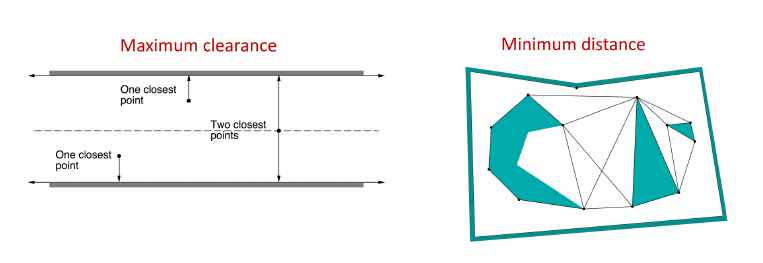
\includegraphics{fig15_6.PNG}
\caption{Other Cell Decomposition Methods Based on Requirements.}
\end{center}
\end{figure}

/subsection{3D Vertical Decomposition}
Computing cell decomposition is much harder for higher-dimensional cases, though vertical cell decomposition is straightforward in 2D. We consider the special case where Cobs is piecewise linear and polyhedral.
It turns out that we can extend the 2D vertical decomposition method by applying the idea of plane-sweeping to higher dimensions. Plane-sweeping refers to sweeping a plane across the space, only to stop where critical change occurs in information. In 3D, assume a polyhedral robot can translate in R3, and the obstacles are polyhedral. Thus Cobs R3 is polyhedral as well. The 3D vertical decomposition algorithm is as follows, as demonstrated in Figure 15.7.

Let (x, y, z) denotes a point in R3. Vertical decomposition yields 3-cell, 2-cell and 1-cell. A generic 3-cell is bounded by 6 planes, and its cross section for a fixed x yields a trapezoid or triangle in a plane parallel to the yz plane. Two sides of a 3-cell are parallel to the yz plane, and two other sides parallel to xz plane. The 3-cell is bounded above and below by two polygonal faces of Cobs.

The general idea is to sweep a plane perpendicular to x axis, where each fixed value of x produces a 2D polygonal slice of Cobs. Three example slices are shown in the bottom of Figure 15.7. Each slice is parallel to yz plane and simplify the 3D problem to a problem that can be solved by 2D vertical decomposition method. The middle slice shows the condition where the sweeping plane just encounters a vertex of a convex polyhedron, represented as a dot. This corresponds to an x value in interest, as critical change
must occur in the slices. Hence, the 3D cell decomposition can be developed incrementally by sweeping through planes to update 2D vertical cell decomposition, in order to incorporate critical changes. To construct a roadmap, sample points are placed at center of each 3-cell and 2-cell. Edges are added to the roadmap by connecting each 3-cell to an adjacent 2-cell.

\section{Graph-Search Algorithms}
Suppose that our environment map has been converted into a connectivity graph using one of the graph generation methods presented earlier. Whatever map representation is chosen, the goal of path planning is to find the best path in the map’s connectivity graph between the start and the goal, where best refers to the selected optimization criteria. In this section, we present several search algorithms that have become
quite popular in mobile robotics.

\begin{figure}[h]
\begin{center}
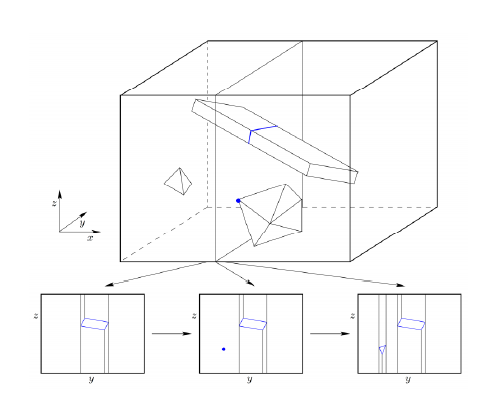
\includegraphics{fig15_7.PNG}
\caption{3D Cell Decomposition Extended from 2D.}
\end{center}
\end{figure}

\subsection{Concepts in graph search}
We introduce the concepts which are all function of the node n (and an adjacent node n0).
g(n) : Path cost(accumulated cost from the start node to any given node n)
c(n, n0) : Edge traversal cost(cost from a node n to an adjacent node n0)
h(n) : Heuristic cost(expected cost from a node n to the goal node)
f (n) : Expected total cost(from start to goal via state n)
f (n) = g(n) + eh(n), where e is a parameter that assumes algorithm-dependent values.

\subsection{Discriminator graph search}
Heuristic function unemployed
– Uniform traversal cost simpler form, obtain faster execution speeds 
ex) depth-first, breadth-first
– Nonuniform traversal cost higher algorithmic complexity
ex) Dijkstra’s algorithm
- Heuristic function employed incorporates additional information about the problem set and thus often allows for faster convergence of the search query.
ex) e = 1 : optimal A* algorithm, e > 1 : suboptimal or greedy A* variant

\subsection{Various graph search algorithms}
Depth-First Search
Depth-first search expands each node up to the deepest level of the graph, until the node has no more successors. As those nodes are expanded, their branch is removed from the graph and the search backtracks by expanding the next neighboring node of the start node until its deepest level and so on.
Depth-First Search stores only a single path from the start nodes for each node on the path, leading to a lower memory requirement. However, previously visited nodes might be visited and the algorithm might enter redundant paths.

\begin{figure}[h!]
\begin{center}
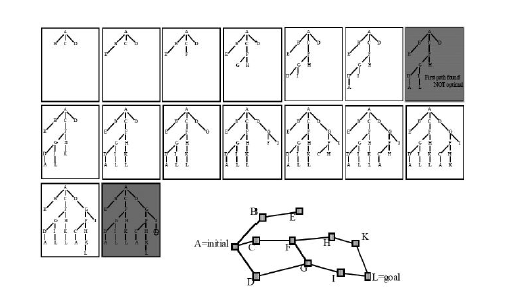
\includegraphics{fig15_8.PNG}
\caption{Depth First Search}
\end{center}
\end{figure}

Breadth-First Search
Breadth-first begins with the start node and explores all of its neighboring nodes. Then, for each of these nodes, it explores all their unexplored neighbors and so on.
The search always returns the path with the fewest number of edges between the start and goal node.

\begin{figure}[h!]
\begin{center}
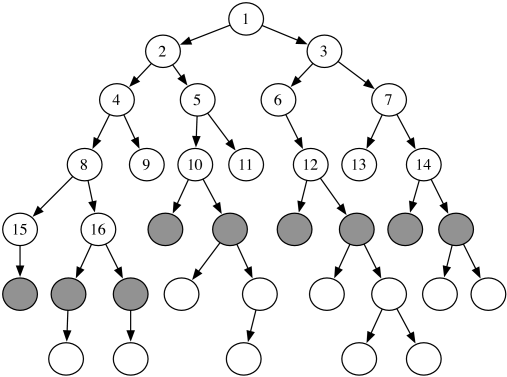
\includegraphics{fig15_9.PNG}
\caption{Breadth First Search}
\end{center}
\end{figure}

Dijkstra’s algorithm (Best-First Search)
Dijkstra’s algorithm is similar to Breadth-First search, except that edge costs may assume any positive value and the search still guarantees solution optimality. Dijkstra’s algorithm uses the concept of the heap, a specialized tree-based data structure and selects the next q as: q = argminq2QC(q))

\subsection{Label Correcting Algorithm}
The label-correction algorithm is a general type of shortest path algorithm which includes very common graph search algorithms like breadth-first search, depth-first search, A*, Dijkstra’s algorithm as special cases.
The idea is to progressively discover shorter paths from the origin to every other node q, and to maintain the lowest cost path(from qI to q) found so far in a variable C(q).

\begin{figure}[h]
\begin{center}
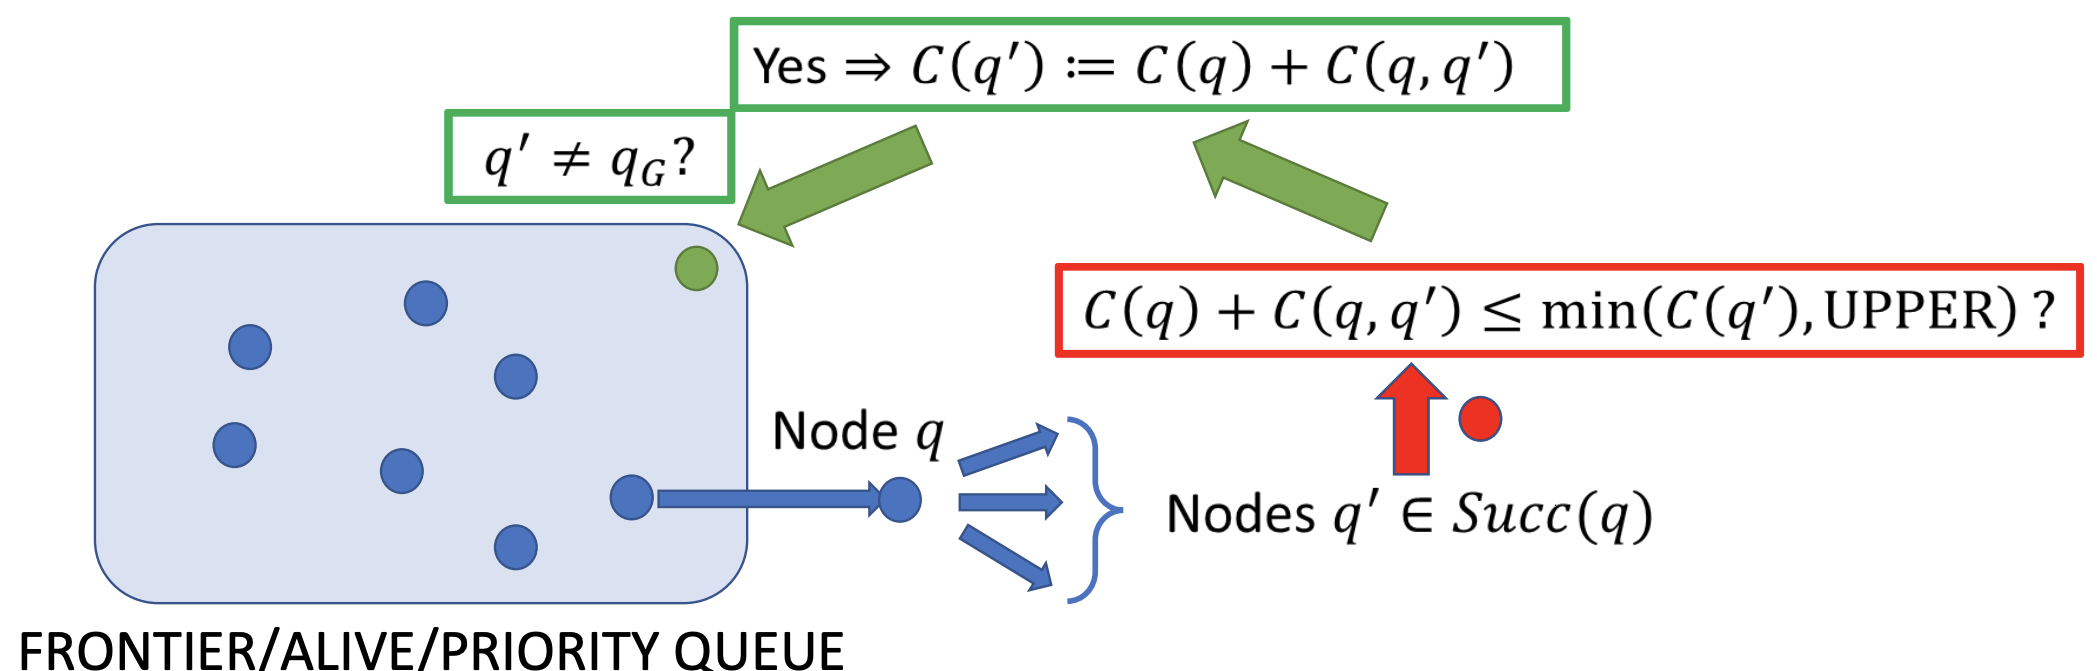
\includegraphics{fig15_10.PNG}
\caption{Label Correcting}
\end{center}
\end{figure}

Algorithm Step
Step1. Remove a node q from the frontier queue and for each child q0 of q, execute step 2
Step2. If C(q) + C(q, q0) min(C(q0),UPPER), set C(q0) := C(q) + C(q, q0) and set q to be the parent of q0. In addition, if q0 6= qG, place q0 in frontier queue if it is not already there, while if q0 = qG, set UPPER to the new value C(q) + C(q, qG)
Step3. If the frontier queue is empty, terminate, else go to step 1.
Initialization : set the labels of all nodes to, except for the label of the origin node, which is set to 0.


\section{Correctness and Improvements}
Label correcting algorithms are guaranteed to find the shortest feasible path from an initial state to a goal state, given one exists. This attribute gives rise to the Correctness Theorem. \vspace{-0.5cm}
\paragraph{Theorem} If a feasible path exists from initial state $q_I$ to goal state $q_G$, then the algorithm terminates in finite time with path cost $C(q_G)$ equal to the optimal cost of traversal, $C^*(q_G)$.\\

However, computing this path can be computationally intensive, especially in high-dimensional problems. This challenge arises from an explosion in the number of states expanded during the search procedure. \\

Consider Fig \ref{fig:graph_search}, Depth-First Search and Breadth-First Search algorithms do not greedily select states from a frontier queue for directed expansion. Hence, these algorithms search the configuration space without direction/relatively uniformly without considering the next state's cost or location relative to the goal. Dijkstra's algorithm improves on Depth-First Search and Breadth-First Search by greedily selecting states from the frontier queue based on cost and by not revisiting previously visited states. However, Dijkstra's algorithm does not take the goal state location into account, potentially leading to wasted effort. Concentrating the search in regions closer to the goal state may reduce the number of states expanded during the search, speeding up the motion planning process.

\begin{figure}[h]
\begin{center}
%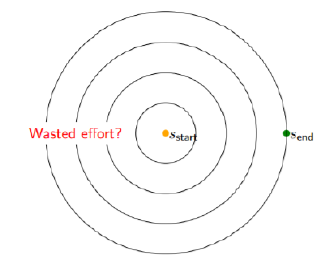
\includegraphics{fig15_11.PNG}
\begin{tikzpicture}[scale=0.9, transform shape]
\draw (0,0) circle (0.6);
% \draw (0,0) circle (1.0);
\draw (0,0) circle (1.2);
% \draw (0,0) circle (2.0);
\draw (0,0) circle (1.8);
\draw (0,0) circle (2.4);

\filldraw[yellow] (0,0) circle (2pt);
\draw (0,0) node[anchor=west] {$s_{\text{start}}$};
\filldraw[green] (2.4,0) circle (2pt);
\draw (2.4,0) node[anchor=west] {$s_{\text{end}}$};

\draw (-3,0) node[anchor=west,color=red] {Wasted Effort?};

\end{tikzpicture}
\caption{Uniform Graph Search Algorithm Exploration}
\label{fig:graph_search}
\end{center}
\end{figure}

\subsection{A*: Improving Dijkstra}
Dijkstra's algorithm orders nodes added to the frontier queue (priority queue) by ``cost-to-arrival" $C(q)$. The A* algorithm (given below) improves on Dijkstra by adding a heuristic function $h(q)$ that models cost to go to the goal state from state $q$, i.e. A* orders by ``cost-to-arrival" + (approximate) ``cost-to-go." This heuristic function, for example distance to goal, guides exploration towards the region of the configuration space close to the goal, leading to faster computations as less states are expanded. Thus, the test
condition changes from
\[ C(q) + C(q, q') \leq \text{UPPER} \qquad
\text{to} \qquad C(q) + C(q, q') + h(q') \leq \text{UPPER}. \] 
The heuristic must be a \textit{positive underestimate} of the true cost to the goal. This modification of the test condition reduces the number of nodes placed in the frontier queue and still guarantees that an optimal path will be returned. In practice, it leads to much faster runtimes.\\

\SetKwInput{KwReturn}{Return}
\begin{algorithm}[H]
\caption{A* Algorithm}
	\KwData{$q_{\text{init}}$, $q_{\text{goal}}$}
	\KwResult{path}
	$C(q) = \infty, \;\; f(q) = \infty\;\; \forall q$\;
	$C(q_{\text{init}}) = 0$, $f(q_{\text{init}}) = h(q_{\text{goal}})$\;
	\tcp{Init frontier queue and explored vertices}
	OPEN = $\{q_{\text{init}}\}$, CLOSED = $\{\}$ \;
	\While{OPEN is not empty}{
	    $q = \argmin_{q' \in \text{OPEN}}f(q')$\;
	    \If{$q$ == $q_{\text{goal}}$}{
	        \KwReturn{path}
	    }
	    OPEN.remove($q$); CLOSE.add($q$)\;
	    \For(\tcp*[f]{Exploration}){$q'$ in \{$q'$ | $(q,q')$ in G, $q'$ not in CLOSED\}}{
	        OPEN.add($q'$)\;
	        \If{$C(q') < C(q) + C(q,q')$}{
	        continue;}
	        $q'$.parent = $q$; $C(q') = C(q) + C(q,q')$\;
	        $f(q') = C(q') + h(q')$
	    }
	}
	\KwReturn{failure}
\end{algorithm}


Figure \ref{fig:astar_example} illustrates A* implemented on a grid. Black states represent obstacles. Yellow states represent nodes in the frontier queue. Blue states represent explored nodes. Green states indicate the final path. The state with the minimum total estimated cost (including the heuristics cost) is selected from the frontier queue for expansion.


\newcolumntype{C}[1]{%
 >{\vbox to 5ex\bgroup\vfill\centering}%
 m{#1}%
 <{\egroup}}  

\newcommand{\stategh}[2]{
\vspace{0.1cm}c={#1}\\ \vspace{0.3cm}h={#2}
}

\newcommand{\stateghblank}[2]{
}

\newcommand{\stateghopen}[2]{
\cellcolor{blue}\vspace{0.1cm}c={#1}\\ \vspace{0.3cm}h={#2}
}

\newcommand{\stateghpq}[2]{
\cellcolor{yellow}\vspace{0.1cm}c={#1}\\ \vspace{0.3cm}h={#2}
}

\newcommand{\stateghpath}[2]{
\cellcolor{green}\vspace{0.1cm}c={#1}\\ \vspace{0.3cm}h={#2}
}

\begin{figure}[h!]
\begin{center}
% 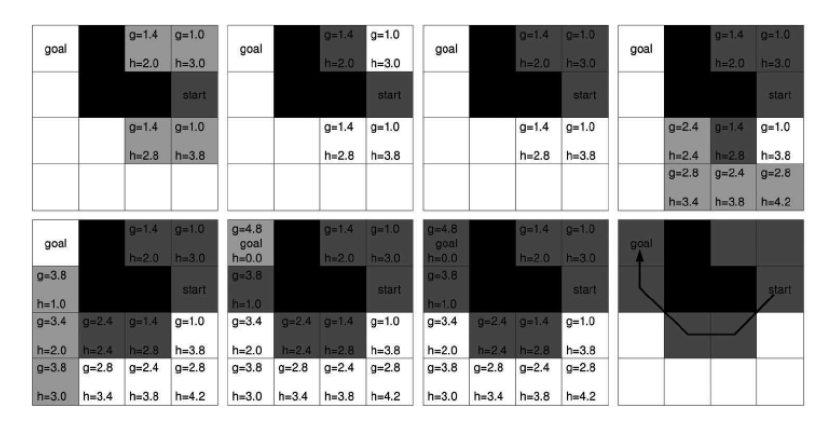
\includegraphics[scale=0.90]{fig15_12.PNG}
\resizebox{.24\columnwidth}{!}{
\begin{tabular}{|C{1cm}|C{1cm}|C{1cm}|C{1cm}|}
    \hline
    goal & \cellcolor{black} & \stateghpq{1.4}{2.0} & \stateghpq{1.0}{3.0}  \tabularnewline
    \hline
    \stateghblank{3.8}{1.0} & \cellcolor{black}& \cellcolor{black} & \cellcolor{blue}{start} \tabularnewline
    \hline
    \stateghblank{3.4}{2.0} & \stateghblank{2.4}{2.4} & \stateghpq{1.4}{2.8} & \stateghpq{1.0}{3.8} \tabularnewline
    \hline
    \stateghblank{3.8}{3.0} & \stateghblank{2.8}{3.4} & \stateghblank{2.4}{3.8} & \stateghblank{2.8}{4.2}\tabularnewline
    \hline
\end{tabular}
}
\resizebox{.24\columnwidth}{!}{
\begin{tabular}{|C{1cm}|C{1cm}|C{1cm}|C{1cm}|}
    \hline
    goal & \cellcolor{black} & \stateghopen{1.4}{2.0} & \stategh{1.0}{3.0}  \tabularnewline
    \hline
    \stateghblank{3.8}{1.0} & \cellcolor{black}& \cellcolor{black} & \cellcolor{blue}{start} \tabularnewline
    \hline
    \stateghblank{3.4}{2.0} & \stateghblank{2.4}{2.4} & \stategh{1.4}{2.8} & \stategh{1.0}{3.8} \tabularnewline
    \hline
    \stateghblank{3.8}{3.0} & \stateghblank{2.8}{3.4} & \stateghblank{2.4}{3.8} & \stateghblank{2.8}{4.2}\tabularnewline
    \hline
\end{tabular}
}
\resizebox{.24\columnwidth}{!}{
\begin{tabular}{|C{1cm}|C{1cm}|C{1cm}|C{1cm}|}
    \hline
    goal & \cellcolor{black} & \stateghopen{1.4}{2.0} & \stateghopen{1.0}{3.0}  \tabularnewline
    \hline
    \stateghblank{3.8}{1.0} & \cellcolor{black}& \cellcolor{black} & \cellcolor{blue}{start} \tabularnewline
    \hline
    \stateghblank{3.4}{2.0} & \stateghblank{2.4}{2.4} & \stategh{1.4}{2.8} & \stategh{1.0}{3.8} \tabularnewline
    \hline
    \stateghblank{3.8}{3.0} & \stateghblank{2.8}{3.4} & \stateghblank{2.4}{3.8} & \stateghblank{2.8}{4.2}\tabularnewline
    \hline
\end{tabular}
}
\vspace{0.3cm}
\resizebox{.24\columnwidth}{!}{
\begin{tabular}{|C{1cm}|C{1cm}|C{1cm}|C{1cm}|}
    \hline
    goal & \cellcolor{black} & \stateghopen{1.4}{2.0} & \stateghopen{1.0}{3.0}  \tabularnewline
    \hline
    \stateghblank{3.8}{1.0} & \cellcolor{black}& \cellcolor{black} & \cellcolor{blue}{start} \tabularnewline
    \hline
    \stateghblank{3.4}{2.0} & \stateghpq{2.4}{2.4} & \stateghopen{1.4}{2.8} & \stategh{1.0}{3.8} \tabularnewline
    \hline
    \stateghblank{3.8}{3.0} & \stateghpq{2.8}{3.4} & \stateghpq{2.4}{3.8} & \stateghpq{2.8}{4.2}\tabularnewline
    \hline
\end{tabular}
}\\
\resizebox{.24\columnwidth}{!}{
\begin{tabular}{|C{1cm}|C{1cm}|C{1cm}|C{1cm}|}
    \hline
    goal & \cellcolor{black} & \stateghopen{1.4}{2.0} & \stateghopen{1.0}{3.0}  \tabularnewline
    \hline
    \stateghpq{3.8}{1.0} & \cellcolor{black}& \cellcolor{black} & \cellcolor{blue}{start} \tabularnewline
    \hline
    \stateghpq{3.4}{2.0} & \stateghopen{2.4}{2.4} & \stateghopen{1.4}{2.8} & \stategh{1.0}{3.8} \tabularnewline
    \hline
    \stateghpq{3.8}{3.0} & \stategh{2.8}{3.4} & \stategh{2.4}{3.8} & \stategh{2.8}{4.2}\tabularnewline
    \hline
\end{tabular}
}
\resizebox{.24\columnwidth}{!}{
\begin{tabular}{|C{1cm}|C{1cm}|C{1cm}|C{1cm}|}
    \hline
    \cellcolor{yellow}goal & \cellcolor{black} & \stateghopen{1.4}{2.0} & \stateghopen{1.0}{3.0}  \tabularnewline
    \hline
    \stateghopen{3.8}{1.0} & \cellcolor{black}& \cellcolor{black} & \cellcolor{blue}{start} \tabularnewline
    \hline
    \stategh{3.4}{2.0} & \stateghopen{2.4}{2.4} & \stateghopen{1.4}{2.8} & \stategh{1.0}{3.8} \tabularnewline
    \hline
    \stategh{3.8}{3.0} & \stategh{2.8}{3.4} & \stategh{2.4}{3.8} & \stategh{2.8}{4.2}\tabularnewline
    \hline
\end{tabular}
}
\vspace{0.3cm}
\resizebox{.24\columnwidth}{!}{
\begin{tabular}{|C{1cm}|C{1cm}|C{1cm}|C{1cm}|}
    \hline
    \cellcolor{blue}goal & \cellcolor{black} & \stateghopen{1.4}{2.0} & \stateghopen{1.0}{3.0}  \tabularnewline
    \hline
    \stateghopen{3.8}{1.0} & \cellcolor{black}& \cellcolor{black} & \cellcolor{blue}{start} \tabularnewline
    \hline
    \stategh{3.4}{2.0} & \stateghopen{2.4}{2.4} & \stateghopen{1.4}{2.8} & \stategh{1.0}{3.8} \tabularnewline
    \hline
    \stategh{3.8}{3.0} & \stategh{2.8}{3.4} & \stategh{2.4}{3.8} & \stategh{2.8}{4.2}\tabularnewline
    \hline
\end{tabular}
}
\resizebox{.24\columnwidth}{!}{
\begin{tabular}{|C{1cm}|C{1cm}|C{1cm}|C{1cm}|}
    \hline
    \cellcolor{green}goal & \cellcolor{black} & \stateghopen{1.4}{2.0} & \stateghopen{1.0}{3.0}  \tabularnewline
    \hline
    \stateghpath{3.8}{1.0} & \cellcolor{black}& \cellcolor{black} & \cellcolor{green}{start} \tabularnewline
    \hline
    \stategh{3.4}{2.0} & \stateghpath{2.4}{2.4} & \stateghpath{1.4}{2.8} & \stategh{1.0}{3.8} \tabularnewline
    \hline
    \stategh{3.8}{3.0} & \stategh{2.8}{3.4} & \stategh{2.4}{3.8} & \stategh{2.8}{4.2}\tabularnewline
    \hline
\end{tabular}
}
\caption{A* Algorithm Example}
\label{fig:astar_example}
\end{center}
\end{figure}


\subsection{Benefits and Drawbacks of Graph-based Approaches}
The graph-based approaches are simple, easy to use, and fast for some problems. However, this approach presents two drawbacks.
\begin{enumerate}
\item These algorithms are resolution dependent, and this resolution is decided a priori. We might find that this resolution is not fine enough to uncover the best path or any path at all for the \textit{original} motion planning problem (for example, if a narrow passage is missed by the discretization).
\item These approaches don't scale well with robot degrees of freedom. Usually, we need to construct a grid with number of dimensions equal to the number of degrees of freedom of our robot. Thus, the number of gird cells increase exponentially, which also increases the number of neighbors of each vertex exponentially in the number of degrees of freedom. Thus, the graph-based approaches become less effective for high dimensional problems (more than 3 DOFs).
\end{enumerate}




\printbibliography

\subsubsection*{Contributors}
Winter 2019: Warren Cheng,  Junwu Zhang, Theo Diamandis\\
Winter 2018: Ryan Richey, Hyoungju Seo, Ola Shorinwa, Josh Sullivan, Danning Sun

\end{document}

